\chapter{Método}

\subsection{Enfoque y tipo}
La investigación se desarrolló bajo un enfoque metodológico mixto (cualitativo-cuantitativo), con predominancia del componente aplicativo-desarrollativo. Se adoptó este enfoque para obtener una comprensión integral del problema: el componente cualitativo permitió profundizar en las percepciones, necesidades y experiencias de los usuarios, mientras que el cuantitativo posibilitó la medición objetiva de variables operativas y de usabilidad. 
El estudio se clasifica como investigación aplicada de tipo tecnológica, dado que su propósito central es el diseño, construcción y validación de un artefacto de software (la plataforma SaaS) para resolver una problemática concreta en un contexto real. El diseño es no experimental, descriptivo y transversal, ya que se observaron y describieron las variables en su contexto natural sin manipulación deliberada, en un período específico.

\section{Diseño de la Investigación}
El presente trabajo sigue la metodología Investigación Basada en Diseño (IBD), elegida por ser es una metodología de investigación poderosa para desarrollar y evaluar artefactos (productos, procesos, métodos, modelos, etc.) que resuelven problemas del mundo real.
No existe un único modelo canónico de fases, ya que distintos autores han propuesto esquemas similares pero con variaciones. Sin embargo, todas comparten un núcleo cíclico y iterativo de construcción y evaluación.
Nosotros presentamos el siguiente esquema integrando los modelos clave de Hevner et al. (2004) y Peffers et al. (2007).

\begin{figure}[htbp]
\centering
\resizebox{\textwidth}{!}{\begin{tikzpicture}[every node/.style={align=center, transform shape, font=\small}, node distance=1.0cm and 2.0cm]
\tikzset{
  phase/.style={draw=black!60, rounded corners=2pt, fill=blue!6, minimum width=5.5cm, minimum height=1.2cm, text width=4.9cm, inner sep=3.5pt},
  phasesmall/.style={draw=black!55, rounded corners=2pt, fill=gray!10, minimum width=5.2cm, minimum height=0.95cm, text width=4.8cm, inner sep=3pt},
  phasediamond/.style={draw=black!60, shape=diamond, aspect=2.2, fill=orange!12, minimum width=5.0cm, minimum height=1.7cm},
  container/.style={draw=black!45, rounded corners=3pt, fill=gray!6, minimum width=14.2cm, minimum height=3.6cm},
  flow/.style={-Latex, draw=black!70, line width=0.5pt},
  arrowlabel/.style={font=\scriptsize, fill=white, fill opacity=0.95, text opacity=1, inner sep=1.6pt, text=black, rounded corners=1pt}
}
\node[container] (ciclo) {};
\node[font=\bfseries, yshift=-0.15cm] at (ciclo.north) {Ciclo iterativo};
\node[phase, anchor=west, xshift=0.35cm, yshift=-0.55cm] at (ciclo.west) (fase3) {Fase 3: Dise\~no \& Desarrollo\\(Construcci\'on del Artefacto)};
\node[phase, anchor=east, xshift=-0.35cm, yshift=-0.55cm] at (ciclo.east) (fase4) {Fase 4: Demostraci\'on\\(Aplicaci\'on/Prueba)};
\draw[flow] (fase3.east) to[bend left=18] node[arrowlabel, midway, yshift=16pt]{Prototipo / Iteraci\'on N} (fase4.west);
\draw[flow] (fase4.west) to[bend left=18] node[arrowlabel, midway, yshift=-16pt]{Feedback / Resultados} (fase3.east);
\node[phasediamond, below=1.4cm of ciclo] (fase5) {Fase 5: Evaluaci\'on};
\draw[flow] (ciclo.south) -- (fase5.north);
\draw[flow] (fase5.east) -- ++(1.0cm,0) coordinate(tmp) -- ++(0,1.0cm) coordinate(tmp2) -- (ciclo.south east) node[midway,right, font=\scriptsize]{No};
\node[phase, below=0.7cm of fase5] (fase6) {Fase 6: Comunicaci\'on \& Difusi\'on};
\draw[flow] (fase5.south) -- node[right, font=\scriptsize]{S\'i} (fase6.north);
\node[phasesmall, below=0.7cm of fase6] (nuevo) {Nuevo Problema o\\Contexto de Aplicaci\'on};
\draw[flow] (fase6.south) -- (nuevo.north);
\node[phase, below=0.7cm of nuevo] (fase1) {Fase 1: Identificaci\'on del Problema};
\draw[flow] (nuevo.south) -- (fase1.north);
\node[phase, below=0.7cm of fase1] (fase2) {Fase 2: Definici\'on de Objetivos};
\draw[flow] (fase1.south) -- (fase2.north);
\draw[flow] (fase2.east) to[out=-10,in=-90] (ciclo.south east);
\end{tikzpicture}
}
\caption{Ciclo iterativo de la Investigación Basada en Diseño}
\label{fig:ibd-ciclo}
\end{figure}

\textbf{Fase 1.} El objetivo de esta fase fue comprender y definir claramente el problema. Se realizó una revisión de la literatura del tema, contextualizándolo en el ámbito global y local.

\textbf{Fase 2.} Una vez comprendido el problema, se establecieron los objetivos que busca conseguir el producto. En esta fase se definieron los requisitos funcionales y no funcionales de la plataforma.

\textbf{Fase 3 y Fase 4.} Forman el ciclo central de construcción-evaluación de la plataforma. Incluye desde la selección de las herramientas tecnológicas, la arquitectura y el desarrollo de la solución. Se trabaja en ciclos cortos.
\begin{itemize}
  \item Se diseña y desarrolla un incremento (un prototipo, una versión, un módulo).
  \item Inmediatamente se demuestra y prueba (en un entorno piloto, con usuarios, en simulación).
  \item Los resultados de esa demostración alimentan directamente el rediseño y desarrollo de la siguiente iteración.
\end{itemize}

\paragraph{Proceso ágil y sprints}
La implementación ágil se estructuró en iteraciones cortas (sprints) con objetivos definidos: levantar requisitos mínimos viables, construir prototipos funcionales, realizar pruebas de usabilidad y ajustar funcionalidades a partir de la retroalimentación. Cada sprint concluyó con una revisión donde se consolidaron mejoras y se definieron tareas para el siguiente ciclo.

\textbf{Fase 5.} Comparar los resultados de la demostración con los objetivos definidos en la Fase 2. Se utilizaron métricas cuantitativas y cualitativas, las mismas que se detallan en la Tabla xx de la sección Técnicas e instrumentos de recolección de datos.

\textbf{Fase 6.} En esta fase se realiza la comunicación de los resultados, los mismos que se definen en la sección Resultados del presente Trabajo.

\subsection{Población y Muestra}

\subsubsection{Población}
La población objetivo estuvo constituida por la totalidad de las Pequeñas y Medianas Empresas (PYMES) del sector gastronómico formalmente establecidas en la ciudad de Portoviejo, provincia de Manabí, Ecuador.
\subsubsection{Muestra y criterios de selección}
Se aplicó un muestreo no probabilístico por conveniencia y criterio. La muestra final estuvo conformada por dos PYMES gastronómicas. Los criterios de inclusión fueron:
\begin{enumerate}[label=\arabic*)]
  \item Ser una PYME ubicada en Portoviejo.
  \item Contar con servicio de consumo en el local y delivery.
  \item Manifestar interés en mejorar procesos mediante digitalización.
  \item Disponer de conectividad básica a internet.
  \item Otorgar consentimiento para participar en todas las fases del estudio.
\end{enumerate}
Se excluyeron establecimientos con operación irregular o que ya utilizaban sistemas de gestión integral.

\subsubsection{Operacionalización de variables}
\textbf{Variable independiente: Plataforma SaaS.} Se define como el artefacto tecnológico desarrollado, una plataforma de Software como Servicio que integra módulos de gestión operativa e inteligencia artificial. Su intervención consistió en su implementación y uso por parte de las PYMES piloto durante el período de validación.

\textbf{Variables dependientes: Indicadores operativos.} Son las métricas de desempeño que se buscó impactar con la implementación de la plataforma:
\begin{enumerate}[label=\arabic*)]
  \item \textbf{Eficiencia en el registro de pedidos:} medida a través del tiempo promedio (minutos) para registrar un pedido y la tasa de errores de registro (porcentaje de pedidos con información incorrecta o incompleta).
  \item \textbf{Eficacia del servicio de delivery:} medida mediante el tiempo promedio de entrega (minutos) desde la confirmación del pedido hasta su entrega.
  \item \textbf{Productividad operativa:} medida a través del volumen diario de pedidos procesados.
  \item \textbf{Calidad del servicio:} inferida a través de la tasa de cancelaciones de pedidos (porcentaje).
  \item \textbf{Usabilidad del sistema:} medida a través del puntaje en la System Usability Scale (SUS), que evalúa la facilidad de uso percibida.
\end{enumerate}

\begin{longtable}{p{3.3cm}p{5.0cm}p{4.2cm}p{3.0cm}}
\caption{\textit{Operacionalización de variables e indicadores de medición}} \\
\toprule
\textbf{Variable dependiente} & \textbf{Definición operacional} & \textbf{Instrumento de medición} & \textbf{Umbral de éxito} \\
\midrule
\endfirsthead
\toprule
\textbf{Variable dependiente} & \textbf{Definición operacional} & \textbf{Instrumento de medición} & \textbf{Umbral de éxito} \\
\midrule
\endhead
Eficiencia en el registro de pedidos & Grado de optimización en la captura y procesamiento inicial de un pedido. & Ficha de observación estructurada (registro de tiempos y errores). & Reducción $\geq$ 25\% en el tiempo promedio de registro y en la tasa de errores. \\
Eficacia del servicio de delivery & Capacidad del sistema para gestionar y completar entregas dentro de un tiempo esperado. & Ficha de observación estructurada (registro de tiempos de entrega). & Reducción $\geq$ 15\% en el tiempo promedio de entrega. \\
Productividad operativa & Volumen de pedidos que el negocio puede procesar de manera efectiva en un día. & Registros administrativos generados por la plataforma (conteo de pedidos diarios). & Incremento $\geq$ 10\% en el número promedio de pedidos diarios procesados. \\
Calidad del servicio & Estabilidad y confiabilidad en la ejecución del servicio, minimizando fallas. & Registros administrativos de la plataforma (conteo de pedidos cancelados). & Reducción $\geq$ 20\% en la tasa de cancelaciones de pedidos. \\
Usabilidad del sistema & Grado de facilidad, eficiencia y satisfacción con que los usuarios pueden emplear la plataforma. & Cuestionario estandarizado System Usability Scale (SUS). & Puntaje promedio $\geq$ 68 (umbral de aceptabilidad en la escala SUS). \\
\bottomrule
\end{longtable}
Nota: Los umbrales de éxito para los indicadores operativos (reducción o incremento porcentual) se establecieron con base en expectativas realistas de mejora para un piloto de corto plazo, considerando la magnitud del cambio que justificaría la adopción de la herramienta. El umbral para el SUS se basa en la clasificación estándar de Bangor et al. (2009).
\subsubsection{Técnicas e instrumentos de recolección de datos}

En la siguiente tabla se muestran las técnicas e instrumentos utilizados, definiendo el momento de la aplicación y el público objetivo.

\begin{longtable}{p{2.1cm}p{2.4cm}p{2.9cm}p{3.1cm}p{2.3cm}p{2.3cm}}
\caption{\textit{Técnicas e instrumentos de recolección de datos}} \\
\toprule
\textbf{Técnica} & \textbf{Instrumento} & \textbf{Objetivo} & \textbf{Características} & \textbf{Momento de aplicación} & \textbf{Público objetivo} \\
\midrule
\endfirsthead
\toprule
\textbf{Técnica} & \textbf{Instrumento} & \textbf{Objetivo} & \textbf{Características} & \textbf{Momento de aplicación} & \textbf{Público objetivo} \\
\midrule
\endhead
Entrevista & Guía de entrevista semiestructurada & Profundizar en los procesos operativos, necesidades específicas y expectativas para el levantamiento de requisitos. & Preguntas abiertas organizadas por áreas (pedidos, inventario, delivery). Grabada y transcrita. & Fase 1: Diagnóstico (línea base). & Propietarios de las PYMES. \\
Prueba de usabilidad & Cuestionario SUS (System Usability Scale) & Medir la usabilidad percibida (facilidad de uso, satisfacción) de la plataforma implementada. & 10 ítems con escala Likert de 5 puntos. Versión estandarizada en español. Confiabilidad ampliamente documentada. & Fase 6: Validación (post-intervención). & Usuarios finales de la plataforma (administradores, cajeros, repartidores). \\
Observación estructurada & Ficha de observación de indicadores operativos & Registrar datos cuantitativos objetivos sobre tiempos, errores y volúmenes de los procesos clave. & Diseñada para registrar: tiempos (min), conteo de errores, volumen de pedidos y cancelaciones. & En dos momentos: pre-intervención (línea base) y post-intervención (semana 3). & Procesos operativos de las PYMES piloto (Local A y B). \\
Revisión documental & Checklist de despliegue y registros administrativos & Verificar la correcta implementación técnica y recopilar datos productivos generados por el sistema. & Lista de verificación para servicios en la nube. Explotación de logs y reportes generados por la propia plataforma. & Fase 6: Validación (post-intervención). & Plataforma SaaS desplegada y sus registros automatizados. \\
\bottomrule
\end{longtable}



\subsubsection{Procedimiento}
La aplicación de la metodología Investigación Basada en Diseño (IBD) se detalla en el Diseño de la investigación. En esta sección se profundiza en las Fases 3, 4 y 5 al ser el núcleo del trabajo.

Para una mejor comprensión metodológica, se detallan siguiendo la estructura:
\begin{enumerate}[label=\arabic*)]
  \item Diseño arquitectónico.
  \item Desarrollo.
  \item Implementación y validación.
\end{enumerate}
Este flujo garantizó una transición estructurada desde la conceptualización técnica hasta la evaluación del sistema en un entorno operativo real.

\paragraph{Diseño de la arquitectura del sistema}
\textbf{Stack tecnológico.} Esta etapa se dedicó a la definición de los cimientos tecnológicos y estructurales de la plataforma. A partir de los requisitos funcionales y no funcionales levantados, se realizó un análisis comparativo de tecnologías, frameworks y herramientas para cada capa del sistema. La selección final se basó en criterios de productividad del desarrollador, mantenibilidad a largo plazo, rendimiento, soporte comunitario y adecuación al contexto de las PYMES (recursos limitados, necesidad de soluciones ligeras). Las decisiones clave se resumen en la Tabla 2.

\begin{longtable}{p{2.6cm}p{3.1cm}p{3.2cm}p{4.6cm}}
\caption{\textit{Selección tecnológica para la arquitectura de la plataforma SaaS}} \\
\toprule
\textbf{Capa / Componente} & \textbf{Tecnología seleccionada} & \textbf{Alternativas evaluadas} & \textbf{Criterio de selección principal} \\
\midrule
\endfirsthead
\toprule
\textbf{Capa / Componente} & \textbf{Tecnología seleccionada} & \textbf{Alternativas evaluadas} & \textbf{Criterio de selección principal} \\
\midrule
\endhead
Backend (API y lógica) & NestJS (Node.js/TypeScript) & Express.js (Node.js), Django (Python), Spring Boot (Java) & Arquitectura modular por defecto, tipado estático (TypeScript) para reducir errores, inyección de dependencias integrada y ecosistema robusto para APIs escalables. \\
Base de datos & PostgreSQL & MySQL, MongoDB (NoSQL) & Modelo relacional adecuado para la integridad de datos transaccionales (pedidos, inventario). Balance entre rendimiento, características avanzadas y costo cero (open-source). \\
Aplicación móvil & React Native + Expo & Flutter (Dart), desarrollo nativo (Kotlin/Swift) & Multiplataforma real (iOS/Android desde un solo código), Expo para agilizar ciclo de desarrollo (builds, testing) y acceso a APIs nativas sin complejidad. \\
Panel web admin & Next.js (React) + Tailwind CSS & React (Create React App), Vue.js, Angular & Renderizado híbrido (SSR/CSR) de Next.js para mejor SEO y performance de carga; Tailwind CSS para estilizado ágil y consistente. \\
Autenticación & JWT (JSON Web Tokens) + bcrypt & Sesiones en servidor, OAuth 2.0 (third-party) & Stateless y escalable para APIs REST. Simplicidad de implementación y seguridad suficiente para el alcance del piloto. \\
Contenedorización & Docker & -- & Estandarización del entorno de desarrollo y despliegue, garantizando consistencia entre equipos y facilitando el deployment en la nube. \\
Despliegue backend/DB & VPS (Hetzner) & AWS/Azure (cloud), Railway, Render & Costo-eficiencia y control total del servidor para un piloto, con rendimiento predecible y facturación simple. \\
Despliegue panel web & Vercel & Netlify, GitHub Pages & Integración nativa con Next.js, despliegue automático por Git, CDN global y SSL gratuito, minimizando tareas de DevOps. \\
\bottomrule
\end{longtable}

\subsubsection{Arquitectura de la Plataforma}

Una vez establecidas las herramientas tecnológicas, se definió y estructuró una arquitectura por capas:

\begin{figure}[htbp]
\centering
\resizebox{0.9\textwidth}{!}{\begin{tikzpicture}[
  font=\small,
  box/.style={draw, rectangle, align=center, minimum height=1.0cm, inner sep=6pt, rounded corners=2pt, line width=0.5pt},
  wide/.style={box, minimum width=12.2cm},
  half/.style={box, minimum width=5.8cm},
  line/.style={-{Latex[length=2mm]}, line width=0.5pt},
  layerframe/.style={draw=black!35, rounded corners=3pt, inner sep=10pt},
  layerlabel/.style={font=\bfseries, fill=white, inner sep=2pt},
  usuarios/.style={wide, fill=blue!12, draw=blue!60},
  acceso/.style={half, fill=cyan!10, draw=cyan!60},
  presentacion/.style={half, fill=orange!12, draw=orange!60},
  negocio/.style={wide, fill=purple!10, draw=purple!60},
  datos/.style={wide, fill=green!12, draw=green!60},
  infra/.style={wide, fill=gray!10, draw=black!55}
]

\node[usuarios] (usuarios) {\textbf{Usuarios}\\Cliente / Admin};
\node[acceso, below=9mm of usuarios] (internet) {\textbf{Acceso}\\Internet};

\node[presentacion, below left=10mm and 8mm of internet] (web) {\textbf{Web}\\Panel / Navegador\\(Next.js)};
\node[presentacion, below right=10mm and 8mm of internet] (app) {\textbf{Móvil}\\Cliente / cocina / reparto\\(React Native)};
\node[layerframe, fit=(web) (app)] (layer1) {};
\node[layerlabel, anchor=west] at ([yshift=8pt]layer1.north west) {Capa 1: Presentación};

\node[negocio, below=12mm of layer1] (api) {\textbf{Capa 2: Lógica de negocio}\\Backend API (REST) (NestJS)};
\node[datos, below=9mm of api] (db) {\textbf{Capa 3: Persistencia}\\Base de datos (PostgreSQL)};
\node[infra, below=9mm of db] (infra) {\textbf{Capa 4: Infraestructura}\\VPS (API + BD) / Vercel (web) / Docker};

\draw[line] (usuarios) -- (internet);
\draw[line] (internet) -- (web);
\draw[line] (internet) -- (app);
\draw[line] (web) -- (api);
\draw[line] (app) -- (api);
\draw[line] (api) -- (db);
\draw[line] (db) -- (infra);
\end{tikzpicture}
}
\caption{Arquitectura por capas de la plataforma SaaS}
\label{fig:arquitectura-capas}
\end{figure}
Los componentes principales de la plataforma son:
\begin{itemize}
  \item Aplicación móvil para clientes y repartidores.
  \item Aplicación web para el panel de administración.
  \item Servicios backends con sus respectivas APIs.
\end{itemize}
Para tener un mejor detalle de cada componente, se presenta a continuación la arquitectura de la aplicación móvil, la arquitectura de la aplicación web y el diagrama de la base de datos.

\begin{figure}[htbp]
\centering
\resizebox{0.85\textwidth}{!}{\begin{tikzpicture}[every node/.style={align=center, transform shape}, node distance=1.0cm]
\tikzset{
  layer/.style={draw, rounded corners, minimum width=9.0cm, minimum height=1.1cm},
  ui/.style={layer, fill=blue!12, draw=blue!60},
  nav/.style={layer, fill=cyan!12, draw=cyan!60},
  services/.style={layer, fill=purple!12, draw=purple!60},
  data/.style={layer, fill=orange!15, draw=orange!60}
}
\node[font=\bfseries] (title) {Arquitectura de la aplicación móvil};
\node[ui, below=0.9cm of title] (ui) {Capa de presentación\\React Native + Tamagui};
\node[nav, below=0.8cm of ui] (nav) {Navegación y estado\\React Navigation + estado local};
\node[services, below=0.8cm of nav] (services) {Servicios de aplicación\\Auth, Pedidos, Catálogo};
\node[data, below=0.8cm of services] (data) {Integración de datos\\API REST + almacenamiento local};
\draw[-latex] (ui.south) -- (nav.north);
\draw[-latex] (nav.south) -- (services.north);
\draw[-latex] (services.south) -- (data.north);
\end{tikzpicture}
}
\caption{Arquitectura de la aplicación móvil}
\label{fig:movil-arquitectura}
\end{figure}

\begin{figure}[htbp]
\centering
\resizebox{0.85\textwidth}{!}{\begin{tikzpicture}[every node/.style={align=center, transform shape}, node distance=1.0cm]
\tikzset{
  layer/.style={draw, rounded corners, minimum width=9.0cm, minimum height=1.1cm},
  ui/.style={layer, fill=blue!12, draw=blue!60},
  routing/.style={layer, fill=cyan!12, draw=cyan!60},
  services/.style={layer, fill=purple!12, draw=purple!60},
  data/.style={layer, fill=orange!15, draw=orange!60}
}
\node[font=\bfseries] (title) {Arquitectura del panel web};
\node[ui, below=0.9cm of title] (ui) {Capa de presentación\\Next.js + Tailwind CSS};
\node[routing, below=0.8cm of ui] (routing) {Ruteo y vistas\\Pages, Layouts, Componentes};
\node[services, below=0.8cm of routing] (services) {Servicios de aplicación\\Gestión, Reportes, Usuarios};
\node[data, below=0.8cm of services] (data) {Integración de datos\\API REST + autenticación JWT};
\draw[-latex] (ui.south) -- (routing.north);
\draw[-latex] (routing.south) -- (services.north);
\draw[-latex] (services.south) -- (data.north);
\end{tikzpicture}
}
\caption{Arquitectura del panel web}
\label{fig:web-arquitectura}
\end{figure}

\begin{figure}[htbp]
\centering
\resizebox{0.85\textwidth}{!}{\begin{tikzpicture}[every node/.style={align=center, transform shape}, node distance=1.2cm and 1.4cm]
\tikzset{
  mod/.style={draw, rounded corners, fill=blue!10, minimum width=4.0cm, minimum height=1.6cm},
  client/.style={draw, rounded corners, fill=gray!15, minimum width=3.6cm, minimum height=0.9cm},
  concern/.style={draw, rounded corners, fill=purple!20, minimum width=3.6cm, minimum height=0.9cm},
  dbnode/.style={draw, rounded corners, fill=orange!20, minimum width=6.4cm, minimum height=1.5cm}
}
\node[font=\bfseries] (title) {Arquitectura Backend (NestJS)};

\node[client, below=0.9cm of title] (mobile) {App móvil};
\node[client, right=8.6cm of mobile] (adminweb) {Panel web};

\node[mod, below=1.1cm of mobile] (auth) {Auth\\Controller\\Service\\Repo};
\node[mod, right=of auth] (users) {Users\\Controller\\Service\\Repo};
\node[mod, right=of users] (products) {Products\\Controller\\Service\\Repo};
\node[mod, below=1.0cm of users] (orders) {Orders\\Controller\\Service\\Repo};
\node[mod, right=of orders] (delivery) {Delivery\\Controller\\Service\\Repo};

\node[dbnode, below=1.2cm of orders] (db) {DB (PostgreSQL)};

\node[draw, dashed, rounded corners, inner sep=8pt, fit={(auth) (users) (products) (orders) (delivery)}] (api) {};

\node[concern, left=1.6cm of api.west] (jwt) {JWT strategy};
\node[concern, below=0.7cm of jwt] (config) {Config};
\node[concern, below=0.7cm of config] (validation) {Validation pipe};
\node[concern, right=1.6cm of api.east] (guards) {Guards};
\node[concern, below=0.7cm of guards] (interceptors) {Interceptors};
\node[concern, below=0.7cm of interceptors] (middleware) {Middleware};

\draw[-latex] (mobile.south) -- (auth.north);
\draw[-latex] (adminweb.south) -- (products.north);
\draw[-latex] (adminweb.south) -- (users.north);
\draw[-latex] (auth.south) -- (db.north);
\draw[-latex] (users.south) -- (db.north);
\draw[-latex] (products.south) -- (db.north);
\draw[-latex] (orders.south) -- (db.north);
\draw[-latex] (delivery.south) -- (db.north);
\draw[-latex, dashed] (jwt.east) -- (api.west);
\draw[-latex, dashed] (config.east) -- (api.west);
\draw[-latex, dashed] (validation.east) -- (api.west);
\draw[-latex, dashed] (guards.west) -- (api.east);
\draw[-latex, dashed] (interceptors.west) -- (api.east);
\draw[-latex, dashed] (middleware.west) -- (api.east);
\end{tikzpicture}
}
\caption{Arquitectura modular del backend (NestJS) planificada}
\label{fig:backend-arquitectura}
\end{figure}

\begin{figure}[htbp]
\centering
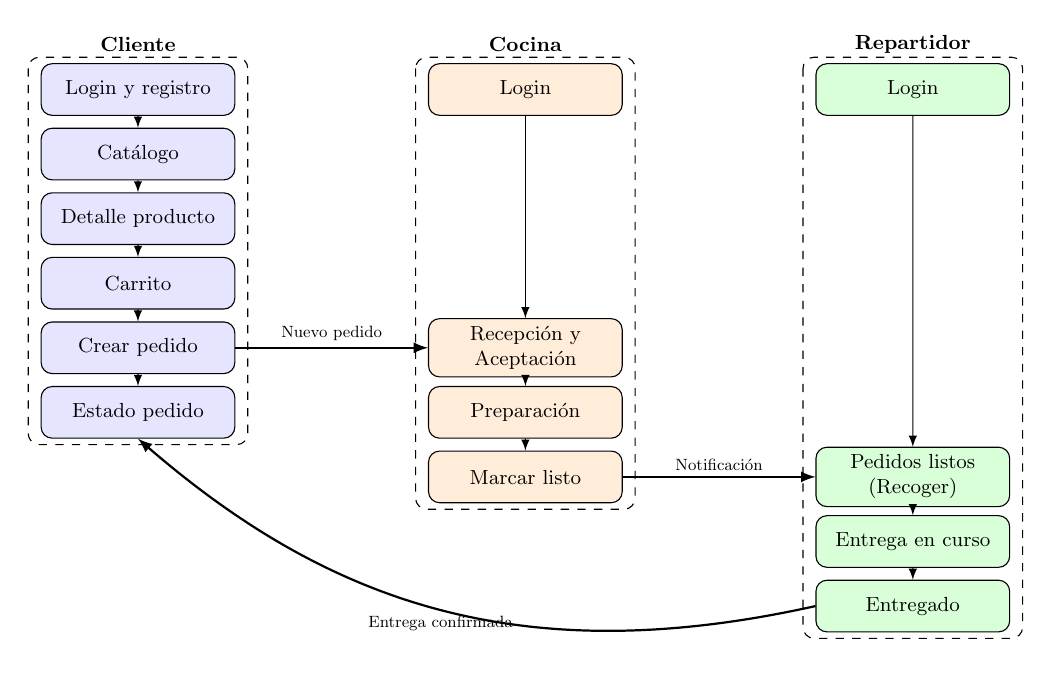
\begin{tikzpicture}[scale=0.82, every node/.style={align=center, transform shape, font=\small}]
\tikzset{
  cstep/.style={draw, rounded corners, fill=blue!10, minimum width=3.0cm, minimum height=0.8cm},
  kstep/.style={draw, rounded corners, fill=orange!15, minimum width=3.0cm, minimum height=0.8cm},
  dstep/.style={draw, rounded corners, fill=green!15, minimum width=3.0cm, minimum height=0.8cm}
}

% Cliente (Left)
\node[cstep] (cl_login) at (-6,4) {Login y registro};
\node[cstep] (cl_catalog) at (-6,3) {Catálogo};
\node[cstep] (cl_detalle) at (-6,2) {Detalle producto};
\node[cstep] (cl_carrito) at (-6,1) {Carrito};
\node[cstep] (cl_crea) at (-6,0) {Crear pedido};
\node[cstep] (cl_estado) at (-6,-1) {Estado pedido};

\draw[dashed, rounded corners] (-7.7,4.5) rectangle (-4.3,-1.5);
\node at (-6,4.7) {\textbf{Cliente}};

\draw[-latex] (cl_login) -- (cl_catalog);
\draw[-latex] (cl_catalog) -- (cl_detalle);
\draw[-latex] (cl_detalle) -- (cl_carrito);
\draw[-latex] (cl_carrito) -- (cl_crea);
\draw[-latex] (cl_crea) -- (cl_estado);

% Cocina (Center)
\node[kstep] (kc_login) at (0,4) {Login};
\node[kstep] (kc_recep) at (0,0) {Recepción y\\Aceptación};
\node[kstep] (kc_prep) at (0,-1) {Preparación};
\node[kstep] (kc_listo) at (0,-2) {Marcar listo};

\draw[dashed, rounded corners] (-1.7,4.5) rectangle (1.7,-2.5);
\node at (0,4.7) {\textbf{Cocina}};

\draw[-latex] (kc_login) -- (kc_recep);
\draw[-latex] (kc_recep) -- (kc_prep);
\draw[-latex] (kc_prep) -- (kc_listo);

% Repartidor (Right)
\node[dstep] (dl_login) at (6,4) {Login};
\node[dstep] (dl_listo) at (6,-2) {Pedidos listos\\(Recoger)};
\node[dstep] (dl_curso) at (6,-3) {Entrega en curso};
\node[dstep] (dl_fin) at (6,-4) {Entregado};

\draw[dashed, rounded corners] (4.3,4.5) rectangle (7.7,-4.5);
\node at (6,4.7) {\textbf{Repartidor}};

\draw[-latex] (dl_login) -- (dl_listo);
\draw[-latex] (dl_listo) -- (dl_curso);
\draw[-latex] (dl_curso) -- (dl_fin);

% Interactions
\draw[-latex, thick] (cl_crea.east) -- node[above, scale=0.8] {Nuevo pedido} (kc_recep.west);
\draw[-latex, thick] (kc_listo.east) -- node[above, scale=0.8] {Notificación} (dl_listo.west);
\draw[-latex, thick] (dl_fin.west) .. controls (0,-5) and (-3,-4) .. node[below, pos=0.5, scale=0.8] {Entrega confirmada} (cl_estado.south);

\end{tikzpicture}

\caption{Diagrama de prototipo del frontend móvil planificado}
\label{fig:frontend-prototipo}
\end{figure}

\begin{figure}[htbp]
\centering
\resizebox{0.9\textwidth}{!}{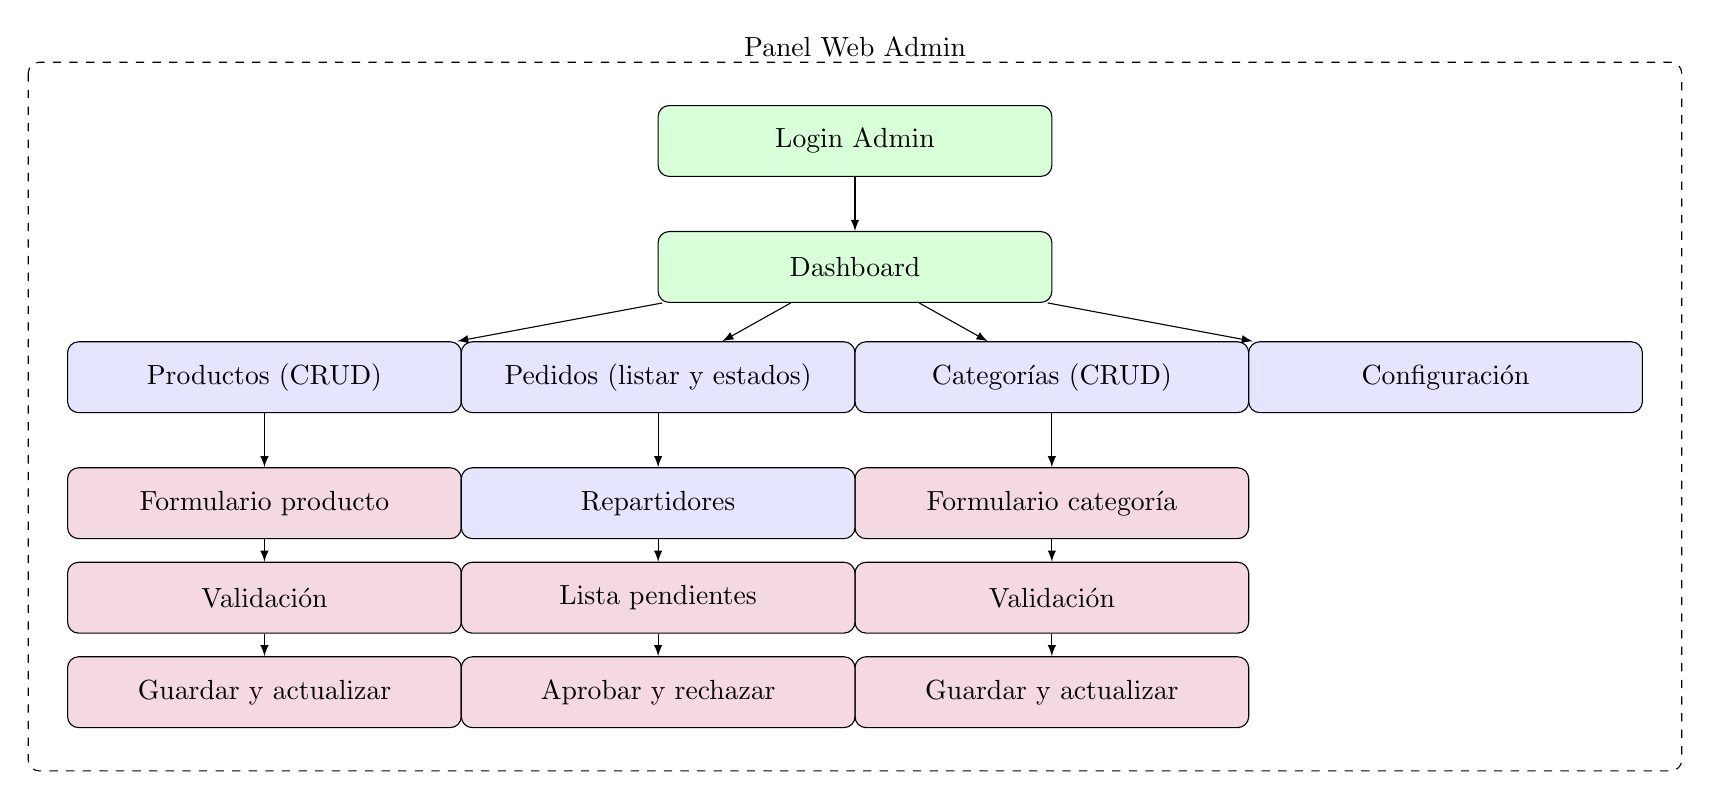
\begin{tikzpicture}[every node/.style={align=center, transform shape}]
\tikzset{
  mod/.style={draw, rounded corners, fill=blue!10, minimum width=5.0cm, minimum height=0.9cm},
  substep/.style={draw, rounded corners, fill=purple!15, minimum width=5.0cm, minimum height=0.9cm}
}
\node[mod, fill=green!15] (login) at (0,0) {Login Admin};
\node[mod, fill=green!15] (dashboard) at (0,-1.6) {Dashboard};
\node[mod] (productos) at (-7.5,-3.0) {Productos (CRUD)};
\node[mod] (pedidos) at (-2.5,-3.0) {Pedidos (listar y estados)};
\node[mod] (categorias) at (2.5,-3.0) {Categorías (CRUD)};
\node[mod] (config) at (7.5,-3.0) {Configuración};

\draw[-latex] (login) -- (dashboard);
\draw[-latex] (dashboard) -- (productos);
\draw[-latex] (dashboard) -- (pedidos);
\draw[-latex] (dashboard) -- (categorias);
\draw[-latex] (dashboard) -- (config);

\node[substep] (prod_form) at (-7.5,-4.6) {Formulario producto};
\node[substep] (prod_valid) at (-7.5,-5.8) {Validación};
\node[substep] (prod_save)  at (-7.5,-7.0) {Guardar y actualizar};
\draw[-latex] (productos) -- (prod_form);
\draw[-latex] (prod_form) -- (prod_valid);
\draw[-latex] (prod_valid) -- (prod_save);

\node[substep] (cat_form) at (2.5,-4.6) {Formulario categoría};
\node[substep] (cat_valid) at (2.5,-5.8) {Validación};
\node[substep] (cat_save)  at (2.5,-7.0) {Guardar y actualizar};
\draw[-latex] (categorias) -- (cat_form);
\draw[-latex] (cat_form) -- (cat_valid);
\draw[-latex] (cat_valid) -- (cat_save);

\node[mod] (repartidores) at (-2.5,-4.6) {Repartidores};
\node[substep] (rep_list)   at (-2.5,-5.8) {Lista pendientes};
\node[substep] (rep_action) at (-2.5,-7.0) {Aprobar y rechazar};
\draw[-latex] (repartidores) -- (rep_list);
\draw[-latex] (rep_list) -- (rep_action);
\draw[-latex] (pedidos) -- (repartidores);
\draw[dashed, rounded corners] (-10.5,1.0) rectangle (10.5,-8.0);
\node at (0,1.2) {Panel Web Admin};
\end{tikzpicture}
}
\caption{Diagrama de prototipo del panel web administrativo planificado}
\label{fig:web-prototipo}
\end{figure}

\subsubsection{Modelo de datos (diseño entidad-relación)}
El modelo entidad-relación que guía la implementación se definió en esta fase. Las entidades principales son: Usuario (id, nombre, email, contraseña encriptada, rol, estado de aprobación para repartidores); Producto (id, nombre, descripción, precio, imagen, asociado a categoría y negocio); Categoría (id, nombre, vinculada al negocio); Pedido (id, fecha/hora, estado, cliente, repartidor asignado), con detalle en tabla OrderItem; Negocio (id, nombre, branding, contacto, configuraciones). En enfoque multinegocio, las entidades incluyen referencia al negocio propietario. El diagrama se presenta en la Figura \ref{fig:er-diagrama}.

\begin{figure}[htbp]
\centering
\resizebox{\textwidth}{!}{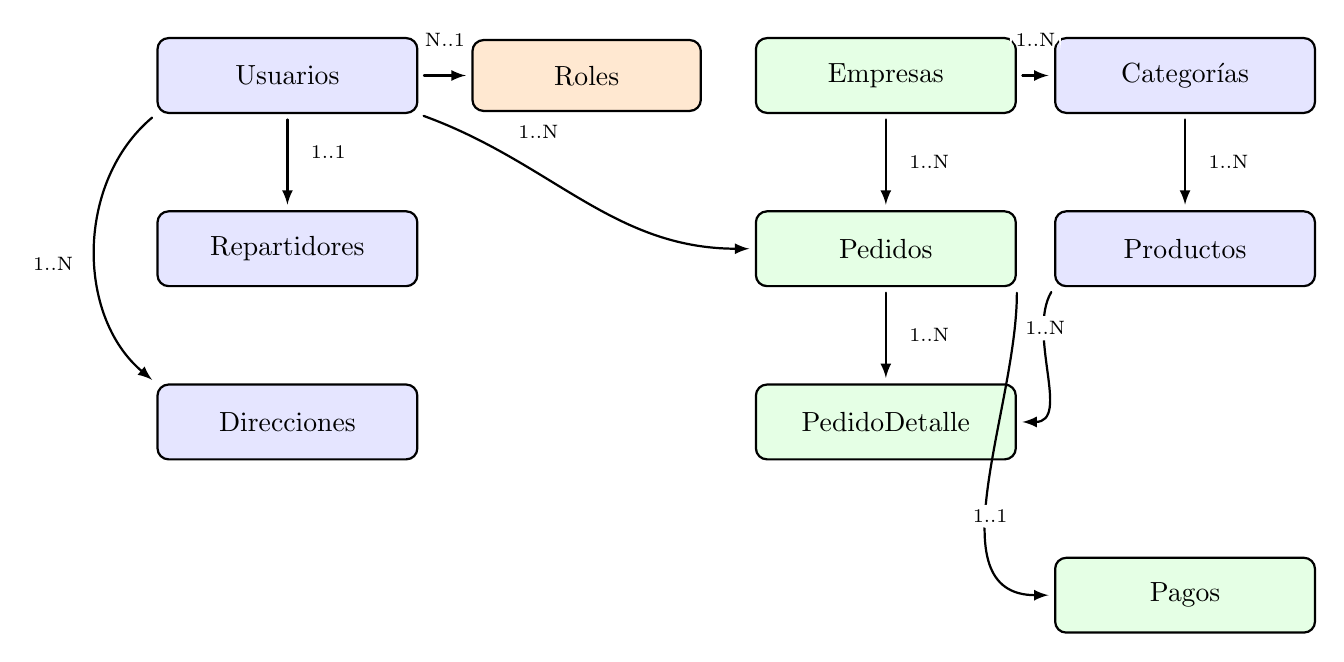
\begin{tikzpicture}[x=3.8cm, y=2.2cm, every node/.style={align=center, transform shape}]
\tikzset{
  entity/.style={draw, rounded corners, thick, fill=blue!10, minimum width=3.3cm, minimum height=0.95cm},
  entityalt/.style={draw, rounded corners, thick, fill=green!10, minimum width=3.3cm, minimum height=0.95cm},
  link/.style={draw, rounded corners, thick, fill=orange!18, minimum width=2.9cm, minimum height=0.9cm},
  relabel/.style={font=\scriptsize, fill=white, inner sep=2pt, outer sep=0.5pt},
  relation/.style={-latex, thick, rounded corners=8pt, line cap=round, line join=round, shorten <=2pt, shorten >=2pt}
}
\node[entity] (usuarios) at (0,2) {Usuarios};
\node[link] (roles) at (1,2) {Roles};
\node[entityalt] (empresas) at (2,2) {Empresas};
\node[entity] (categorias) at (3,2) {Categorías};
\node[entity] (repartidores) at (0,1) {Repartidores};
\node[entity] (direcciones) at (0,0) {Direcciones};
\node[entityalt] (pedidos) at (2,1) {Pedidos};
\node[entity] (productos) at (3,1) {Productos};
\node[entityalt] (pedidoDetalle) at (2,0) {PedidoDetalle};
\node[entityalt] (pagos) at (3,-1) {Pagos};

\draw[relation] (usuarios) -- node[relabel, above, pos=0.5, yshift=8pt] {N..1} (roles);
\draw[relation] (usuarios) -- node[relabel, right, pos=0.4, xshift=6pt] {1..1} (repartidores);

\draw[relation] (usuarios.south west) to[out=-140,in=140] node[relabel, left, pos=0.55, xshift=-6pt] {1..N} (direcciones.north west);
\draw[relation] (usuarios.south east) to[out=-20,in=180] node[relabel, above, pos=0.35, yshift=10pt] {1..N} (pedidos.west);

\draw[relation] (empresas.south) -- node[relabel, right, pos=0.5, xshift=6pt] {1..N} (pedidos.north);
\draw[relation] (empresas) -- node[relabel, above, pos=0.5, yshift=8pt] {1..N} (categorias);

\draw[relation] (categorias) -- node[relabel, right, pos=0.5, xshift=6pt] {1..N} (productos);

\draw[relation] (pedidos) -- node[relabel, right, pos=0.5, xshift=6pt] {1..N} (pedidoDetalle);
\draw[relation] (productos.south west) to[out=-120,in=0] node[relabel, above, pos=0.45, yshift=8pt] {1..N} (pedidoDetalle.east);
\draw[relation] (pedidos.south east) to[out=-90,in=180] node[relabel, below, pos=0.5, yshift=-6pt] {1..1} (pagos.west);
\end{tikzpicture}
}
\caption{Diagrama entidad-relación (ER) del esquema de datos planificado}
\label{fig:er-diagrama}
\end{figure}

\subsection{FASE 2: Desarrollo}
En esta fase se implementó la plataforma siguiendo la arquitectura, las tecnologías y los diseños definidos en la Fase 1. A continuación se describe cómo quedó estructurado el software en módulos y componentes.

\subsubsection{Implementación del frontend móvil (React Native + Expo)}
El frontend móvil se construyó según el prototipo planificado (Figura \ref{fig:frontend-prototipo}), utilizando React Native y Expo \parencite{campusmvp_expo}. La aplicación organiza sus pantallas en flujos diferenciados para los roles Cliente y Repartidor, además de inicio de sesión y registro. La navegación se gestiona con React Navigation; cada rol visualiza únicamente las opciones pertinentes, con validaciones en el backend. La comunicación con la API se realiza mediante HTTP y JSON; se contemplan errores de conectividad y respuestas 4xx/5xx con mensajes claros. Para la interfaz se empleó Tamagui \parencite{tamagui_github}, con formularios controlados y validación básica en cliente.

La arquitectura del frontend móvil privilegia la simplicidad y la previsibilidad del estado. Se emplea estado local y patrones de elevación de estado donde corresponde, con manejo de formularios controlados y validación básica en cliente (tipos de entrada, obligatoriedad, formatos).

La comunicación con la API se realiza mediante solicitudes HTTP que envían y reciben JSON; se contemplan casos de error (credenciales inválidas, falta de conectividad, respuestas 4xx/5xx) con mensajes claros al usuario y estrategias de reintento cuando es pertinente.

La interfaz se diseñó con principios de consistencia visual y accesibilidad, cuidando contrastes, tamaños de toque y retroalimentación tras acciones.

\subsubsection{Implementación del panel web (Next.js + Tailwind CSS)}
El panel administrativo se implementó según el prototipo definido en la Fase 1 (Figura \ref{fig:web-prototipo}), con React, Next.js y Tailwind CSS \parencite{tailwind_es}. La estructura de navegación organiza secciones por dominio (productos, categorías, pedidos, repartidores) con filtros por estado y fecha. El panel permite crear y editar productos, gestionar categorías y aprobar o rechazar repartidores; los formularios incorporan validaciones y las vistas de lista presentan pedidos en curso y solicitudes pendientes. Se aprovechó SSR en vistas de dashboard cuando resultó conveniente. Ambos frontends consumen el mismo backend mediante API REST y JSON.

En el panel se aplicaron formularios validados con reglas de negocio simples (campos requeridos, formatos, rangos) y se implementaron flujos habituales de CRUD con confirmaciones y mensajes de éxito/error.

La estructura de navegación organiza secciones por dominio (productos, categorías, pedidos, repartidores) y proporciona filtros básicos (por estado, fecha) para facilitar la gestión. Se cuidó la responsividad para operar en distintos tamaños de pantalla, y se diseñaron tablas y listas con paginación prevista para escenarios de datos voluminosos.

El panel permite crear y editar productos, gestionar categorías y aprobar o rechazar repartidores que solicitan unirse. Los formularios incorporan validaciones de campos; las vistas de lista presentan pedidos en curso y solicitudes pendientes.

Cuando un repartidor se registra desde la app móvil, su cuenta queda "pendiente" hasta la revisión administrativa, tras la cual puede ser habilitada o rechazada, garantizando control de calidad.

Ambos frontends consumen el mismo backend mediante API REST y JSON. La separación de responsabilidades mantiene el frontend enfocado en la experiencia y presentación, mientras la lógica de negocio y la persistencia residen en el backend.

En materia de rendimiento y experiencia, se optimizaron listas y vistas frecuentes y se cuidó la retroalimentación visual en operaciones que pueden tardar (carga de catálogo, envío de pedidos).

Se delinearon buenas prácticas para el manejo de imágenes (compresión, tamaños adecuados) y para el control de estados vacíos y errores de red, mejorando la robustez de la interfaz en condiciones reales.

\subsubsection{Implementación del backend (NestJS, módulos)}
El backend se implementó según la arquitectura planificada en la Fase 1 (Figura \ref{fig:backend-arquitectura}), con NestJS y TypeScript \parencite{dragosb_lo_mejor_nestjs}. La aplicación se organiza en los siguientes módulos: Auth (login, registro, JWT); Users (usuarios y roles); Products y Categories (catálogo); Orders (creación, asignación y estados de pedidos); Delivery (operativas de repartidores). Cada módulo agrupa controlador (endpoints HTTP), servicio (lógica de negocio) y capa de datos (TypeORM). Se emplean DTOs con class-validator para validación de entrada, pipes globales, filtros de excepciones y Guards (JwtAuthGuard, RolesGuard). La persistencia se maneja con TypeORM sobre PostgreSQL; la configuración se lee de variables de entorno (ConfigModule). Para despliegue se contempló Docker y un servidor en la nube (Hetzner \parencite{hetzner_cloud}); la arquitectura de despliegue se presenta en la Figura \ref{fig:despliegue-arquitectura}.

\subsubsection{Implementación del modelo de datos}
El modelo entidad-relación definido en la Fase 1 (Figura \ref{fig:er-diagrama}) se implementó con TypeORM: cada entidad se refleja en una clase con decoradores @Entity; las relaciones se anotan con @ManyToOne, @OneToMany, etc. Se adoptó el modelo compartido con discriminador \texttt{businessId} en tablas relevantes para multinegocio \parencite{scalzotto_multitenancy_nestjs}. Las consultas filtran por negocio del usuario autenticado; se definieron índices en campos de búsqueda frecuente y restricciones de unicidad. En operaciones compuestas (creación de pedido y detalle) se contemplan transacciones.

\subsubsection{Roles, permisos y seguridad (JWT, RBAC)}
La plataforma implementa un esquema de roles y permisos (RBAC) para garantizar que cada usuario solo realice las acciones que le corresponden \parencite{logto_rbac_docs}. RBAC gestiona "quién puede hacer qué" agrupando permisos en roles; a cada usuario se le asigna uno o varios roles y cada rol confiere permisos sobre funciones, APIs o datos.

Administrador (ADMIN): Usuario del panel web con privilegios completos. Puede crear y editar productos y categorías, ver todos los pedidos, gestionar repartidores (aprobar/rechazar) y configurar la plataforma. En entornos multinegocio podría existir un administrador por empresa.

Cliente (CLIENTE): Usuario de la app móvil que realiza pedidos. Puede registrarse o iniciar sesión, ver y buscar productos, crear pedidos, consultar su estado y editar su perfil.

Repartidor (DELIVERY): Usuario de la app móvil que toma y entrega pedidos. Puede ver pedidos pendientes, aceptar/declinar encargos, marcar entregas y revisar su historial. Requiere aprobación administrativa antes de operar.
Estos roles se asignan en la base de datos, ya sea mediante un campo role en la tabla de usuarios o mediante una relación muchos a muchos Usuario-Rol (si quisiéramos soportar múltiples roles por usuario). En este proyecto, dado que los roles son bien diferenciados, optamos por un campo simple enumerado ('ADMIN' | 'CLIENTE' | 'DELIVERY') en la entidad Usuario para la simplicidad.

La autorización por roles se implementa de forma declarativa en endpoints críticos, con mensajes de error consistentes y registro de intentos no autorizados para auditoría. En cuanto a autenticación, se definieron políticas de expiración de tokens equilibradas entre seguridad y usabilidad; por simplicidad, inicialmente no se emplean tokens de actualización (refresh), aunque se prevé su inclusión si el uso lo amerita. Se recomienda almacenar credenciales y tokens de forma segura en cliente (cookies HttpOnly en web, almacenamiento seguro en móvil) y evitar exposición en logs.
\begin{figure}[htbp]
\centering
\resizebox{0.9\textwidth}{!}{\begin{tikzpicture}[every node/.style={align=center, transform shape, font=\footnotesize}, node distance=0.6cm and 1.6cm]
\tikzset{
  box/.style={draw, rounded corners=2pt, fill=blue!15, minimum width=2.8cm, minimum height=0.7cm, line width=0.6pt},
  token/.style={draw, rounded corners=2pt, fill=cyan!20, minimum width=2.4cm, minimum height=0.7cm, line width=0.6pt},
  stepbox/.style={draw, rounded corners=2pt, fill=orange!25, minimum width=2.8cm, minimum height=0.65cm, line width=0.6pt},
  group/.style={draw, dashed, rounded corners=4pt, inner sep=3pt, line width=0.6pt},
  flow/.style={-Latex, line width=0.6pt, shorten <=2pt, shorten >=2pt}
}
\node[box] (client) {Cliente App};
\node[box, below=of client] (login) {POST /auth/login};
\node[token, below=of login] (jwt) {JWT};
\node[group, fit=(client) (login) (jwt)] (grpAuth) {};
\node at ([yshift=6pt] grpAuth.north) {Autenticación};

\node[box, right=2.1cm of login] (endpoint) {Endpoint protegido};
\node[stepbox, below=of endpoint] (authguard) {AuthGuard [jwt]};
\node[stepbox, below=of authguard] (rolesguard) {RolesGuard\\(RBAC)};
\node[stepbox, below=of rolesguard] (controller) {Controller};
\node[stepbox, below=of controller] (service) {Service};
\node[stepbox, below=of service] (response) {Respuesta};
\draw[flow] (client.south) -- (login.north) node[midway, right] {HTTPS};
\draw[flow] (login.south) -- (jwt.north) node[midway, right] {Bearer};
\draw[flow] (jwt.east) -- (endpoint.west);
\draw[flow] (endpoint.south) -- (authguard.north);
\draw[flow] (authguard.south) -- (rolesguard.north);
\draw[flow] (rolesguard.south) -- (controller.north);
\draw[flow] (controller.south) -- (service.north);
\draw[flow] (service.south) -- (response.north);
\node[group, fit=(endpoint) (authguard) (rolesguard) (controller) (service) (response)] (grpAPI) {};
\node at ([yshift=6pt] grpAPI.north) {Autorización y API};
\node[draw, circle, fill=gray!15, minimum size=0.65cm, right=0.5cm of rolesguard] (roleAdmin) {Admin};
\node[draw, circle, fill=gray!15, minimum size=0.65cm, below=0.15cm of roleAdmin] (roleClient) {Cliente};
\draw[dashed] (rolesguard.east) -- (roleAdmin.west);
\draw[dashed] (rolesguard.east) -- (roleClient.west);
\end{tikzpicture}
}
\caption{Flujo de autenticación y autorización}
\label{fig:auth-rbac}
\end{figure}
Para la autenticación y autorización, utilizamos JWT (JSON Web Tokens) como mecanismo de autenticación stateless. JWT es un estándar abierto (RFC 7519) ampliamente utilizado para transmitir información de forma segura en forma de token JSON firmado. De hecho, la autenticación con tokens JWT se ha convertido en un estándar de facto para proteger los endpoints sensibles de aplicaciones web y APIs \parencite{raguilera_jwt_nestjs}. En nuestro sistema, implementamos JWT mediante la integración de Passport.js en NestJS con la estrategia passport-jwt.

El flujo es el siguiente:
\begin{enumerate}[label=\arabic*.]
  \item Un usuario se registra (para nuevos clientes/repartidores) o inicia sesión proporcionando sus credenciales (email/usuario y contraseña).
  \item El servidor NestJS valida esas credenciales contra la base de datos (la contraseña almacenada está encriptada con bcrypt; durante el login se compara el hash). Si son correctas, el servidor genera un token JWT firmado con nuestra clave secreta y se lo devuelve al cliente.
  \item Este token incluye en su payload datos básicos del usuario, típicamente su identificador único de usuario y su rol. No incluimos información sensible en el JWT ya que viaja en claro (solo firmado, no cifrado) \parencite{raguilera_jwt_nestjs}; únicamente identificadores y claims necesarios para autorización.
  \item El cliente (app móvil o panel web) almacena este token, generalmente en memoria o almacenamiento local seguro (en el caso de la app, Expo SecureStore u AsyncStorage; en el caso web, cookies HttpOnly o localStorage con cuidado). En cada petición subsecuente a la API que requiera autenticación, el cliente envía el token en la cabecera Authorization: Bearer.
  \item El backend, gracias a Passport JWT, intercepta esas peticiones protegidas: la estrategia JWT extrae el token de la cabecera y lo verifica (comprueba firma y validez). Si es válido, decodifica el payload y adjunta esa info del usuario en el objeto Request (por ej., req.user).
\end{enumerate}

A partir de ahí, los Guards de NestJS determinan si se permite o deniega el acceso:
\begin{itemize}
  \item Primero, usamos un guard genérico \texttt{JwtAuthGuard} (que extiende de \texttt{AuthGuard('jwt')} de Nest) para verificar la autenticación. Este guard está aplicado a todas las rutas que requieren un usuario logueado.
  \item Si el token es inválido o expiró, el guard rechaza la petición automáticamente con código 401 Unauthorized.
  \item Personalización mínima: extender \texttt{AuthGuard('jwt')} y, en \texttt{handleRequest}, si existe error o no hay usuario, lanzar \texttt{UnauthorizedException} con el mensaje en español: “No autorizado. Por favor, inicie sesión”. En caso contrario, retornar el usuario.
\end{itemize}
Este guard utiliza internamente la estrategia JWT definida (la cual, en nuestro AuthService, valida el token y puede que re-fresque algunos datos del usuario si es necesario). Al implementar handleRequest, nos aseguramos de capturar los casos en que Passport no encuentre usuario (token inválido) para siempre lanzar nuestra excepción personalizada \parencite{creapolis_nestjs_2025,dragosb_lo_mejor_nestjs}. De esta manera, ningún endpoint sensible será ejecutado sin un JWT válido.
En segundo lugar, para la autorización por roles (RBAC) se implementó un guard adicional, por ejemplo RolesGuard, combinado con un decorador personalizado @Roles(...) que se añade a controladores o métodos indicando los roles permitidos. Al ejecutarse, RolesGuard lee los metadatos requeridos y los compara con el rol de \texttt{req.user} (poblado por JwtAuthGuard). Si el usuario no cumple, se lanza un Forbidden (403). Este patrón recomendado por NestJS — definir un guard genérico y roles por ruta con metadatos — mejora legibilidad y reduce errores \parencite{stackoverflow_roleguards}. Por ejemplo:
Declaración mínima por ruta: \texttt{@UseGuards(JwtAuthGuard, RolesGuard)} junto con \texttt{@Roles('ADMIN')} en endpoints administrativos asegura acceso exclusivo a administradores autenticados. De forma análoga, rutas de repartidor se etiquetan con \texttt{@Roles('DELIVERY')}.

Lógica esencial de \texttt{RolesGuard}: obtener metadatos \texttt{'roles'} con \texttt{Reflector}; si no existen, permitir acceso; si existen, comparar \texttt{user.role} contra los roles requeridos y permitir solo en coincidencia; si no, responder con 403. Este enfoque mantiene permisos declarativos y reduce errores de autorización.
Así, añadimos una capa de control de acceso declarativo: los permisos de cada endpoint están explícitos vía decoradores, lo que mejora la legibilidad y reduce errores de permiso.
En términos de seguridad de datos, las contraseñas se almacenan con hashing \texttt{bcrypt} y \textit{salt} aleatorio. Al registrar un usuario, la contraseña se encripta; al validar credenciales en login se usa \texttt{bcrypt.compare()} contra el hash guardado, ya sea mediante un hook \texttt{@BeforeInsert} en la entidad de TypeORM o desde el servicio de autenticación.

Los tokens JWT se firman con una clave segura definida en variables de entorno (\texttt{JWT\_SECRET}), usando algoritmo \texttt{HS256}. La expiración se configura (p. ej., 1–7 días) mediante \texttt{signOptions.expiresIn} en \texttt{JwtModule} \parencite{raguilera_jwt_nestjs}, equilibrando seguridad y usabilidad.

El transporte entre frontend y backend se realiza sobre \texttt{HTTPS} para proteger tokens y datos personales.

Las validaciones de negocio verifican contexto y roles en operaciones sensibles; por ejemplo, al marcar entregado, el servicio comprueba \texttt{order.assignedTo == user.id} antes de aceptar el cambio (\texttt{markAsDelivered(orderId, user)}).
Cabe destacar que gran parte de esta infraestructura de seguridad se apalanca en las facilidades de NestJS. La documentación y guías técnicas disponibles describen la integración de JWT y Passport, las cuales seguimos adaptando a nuestras necesidades específicas (como mensajes en español, y la estructura de usuarios/roles propia) \parencite{creapolis_nestjs_2025,dragosb_lo_mejor_nestjs}. Este enfoque modular nos permite extender la seguridad fácilmente: si se quisiera integrar OAuth2 o autenticación con terceros en el futuro, se añadiría otra estrategia Passport sin reescribir todo el auth. O, si se quisiera implementar permisos más granulares (por ejemplo, nivel de recurso), NestJS Guards e interceptors podrían manejarlo.
En resumen, JWT y RBAC son la columna vertebral de la seguridad de nuestra plataforma. JWT brinda una forma stateless de autenticar peticiones – eliminando la necesidad de mantener sesiones en el servidor – y RBAC garantiza que cada endpoint sólo pueda ser usado por los roles adecuados. Este modelo nos da confianza en que, por ejemplo, ningún cliente podrá acceder a los servicios de administración aunque intente manipular la app, y ningún repartidor podrá leer o modificar datos que no le conciernen (como listado de usuarios, o pedidos que no le fueron asignados). La combinación de estas medidas crea una capa de seguridad profunda, desde el almacenamiento cifrado de contraseñas, la autenticación robusta en cada request, hasta la autorización fina por rol y validaciones de negocio adicionales.

\subsubsection{Flujo funcional (proceso de pedido de punta a punta)}
A continuación se describe el flujo funcional de la plataforma, integrando frontend móvil, frontend web, backend, base de datos y roles según el diagrama de secuencia elaborado. El caso típico inicia con el registro del usuario desde la app móvil, donde puede optar por Cliente o aspirante a Repartidor y enviar sus datos mediante \texttt{POST /auth/register}. El backend valida la petición en el controlador de autenticación, crea el usuario en la base de datos y encripta la contraseña; si el registro es de repartidor, se marca como pendiente de aprobación.

Tras el registro, el usuario realiza inicio de sesión con \texttt{POST /auth/login}. Si las credenciales son válidas, el servicio de autenticación genera un JWT firmado con \texttt{userId} y \texttt{role} \parencite{raguilera_jwt_nestjs}, que la app almacena y adjunta en futuras peticiones (\texttt{Authorization: Bearer ...}). En caso de error, se retorna un 401 con mensaje apropiado. Una vez autenticado, el acceso y las vistas dependen del rol.

Como Cliente, la app muestra el catálogo de productos y consulta \texttt{GET /products}. El backend, protegido con JwtAuthGuard, obtiene los productos del servicio, filtrando por negocio si corresponde en contextos multinegocio. El cliente puede buscar por categorías y gestionar un carrito local.

Como Repartidor, si la cuenta está pendiente de aprobación se rechaza el acceso con un mensaje de revisión; una vez aprobado, el repartidor inicia sesión y accede a la lista de pedidos disponibles mediante \texttt{GET /orders/available}, protegida con JwtAuthGuard y RolesGuard('DELIVERY'). El backend devuelve los pedidos en estado pendiente, posiblemente filtrados por negocio.

El Cliente crea un pedido con \texttt{POST /orders} enviando items, cantidades, dirección y notas, autenticado con JWT. El controlador de pedidos pasa por JwtAuthGuard (y, de ser necesario, RolesGuard('CLIENTE')), y el servicio valida productos, calcula totales y persiste la entidad Pedido con estado inicial "Pendiente" y su detalle. La respuesta confirma el pedido y su estado.

La disponibilidad del pedido para repartidores puede propagarse por consulta periódica (polling) o, idealmente, por notificaciones en tiempo real (WebSockets o Expo Notifications). En esta fase se asume refresco manual o polling; el pedido aparece en la lista de disponibles.

Cuando un repartidor acepta un pedido (\texttt{POST /orders/{id}/assign}), el backend verifica que aún no esté asignado y actualiza el estado a "En camino" (o "Asignado"), registrando el usuario asignado. La app de repartidor mueve el pedido a sus entregas activas y el cliente puede ser notificado del cambio de estado.

La entrega se marca con \texttt{POST /orders/{id}/deliver} (o un PATCH equivalente). El backend valida que el pedido esté asignado al repartidor autenticado y en estado correcto, y actualiza a "Entregado" con la hora efectiva. Se pueden calcular métricas como tiempo de entrega en futuras iteraciones. El cliente recibe confirmación y el administrador visualiza los estados desde su panel.

El administrador gestiona repartidores pendientes con \texttt{GET /users?role=DELIVERY\&pending=true} y los aprueba con \texttt{PATCH /users/{id}/approve}, además de administrar catálogo (\texttt{POST /products}, \texttt{POST /categories}, \texttt{PUT /products/{id}}) y revisar pedidos (\texttt{GET /orders}), con posibilidad de intervenir sobre estados (por ejemplo, cancelar con \texttt{PATCH /orders/{id}/cancel}). También puede listar usuarios por rol (\texttt{GET /users?role=CLIENTE}). Con el pedido entregado, el ciclo se cierra: el cliente recibe su producto, el repartidor completa su tarea y el administrador mantiene registro íntegro en la base de datos.

En escenarios de error, el sistema informa de forma clara y recuperable: si fallan credenciales en login, se muestra un mensaje específico; si un pedido ya fue asignado cuando otro repartidor intenta tomarlo, el backend devuelve un error de conflicto y la app actualiza la vista; si la conexión se interrumpe, se sugiere reintentar o se conserva el estado local hasta restablecer comunicación. El diseño contempla fallos previsibles y asegura que no se pierdan datos críticos.

Para mejorar la experiencia, se considera integrar actualizaciones en tiempo real de estado de pedidos en ambas apps y visualizaciones más ricas en el panel admin (por ejemplo, mapas de entregas y colas de pedidos). Aunque actualmente el refresco es manual o por consulta periódica, la arquitectura permite incorporar canales de eventos sin modificar la lógica principal.
\begin{figure}[htbp]
\centering
\resizebox{0.9\textwidth}{!}{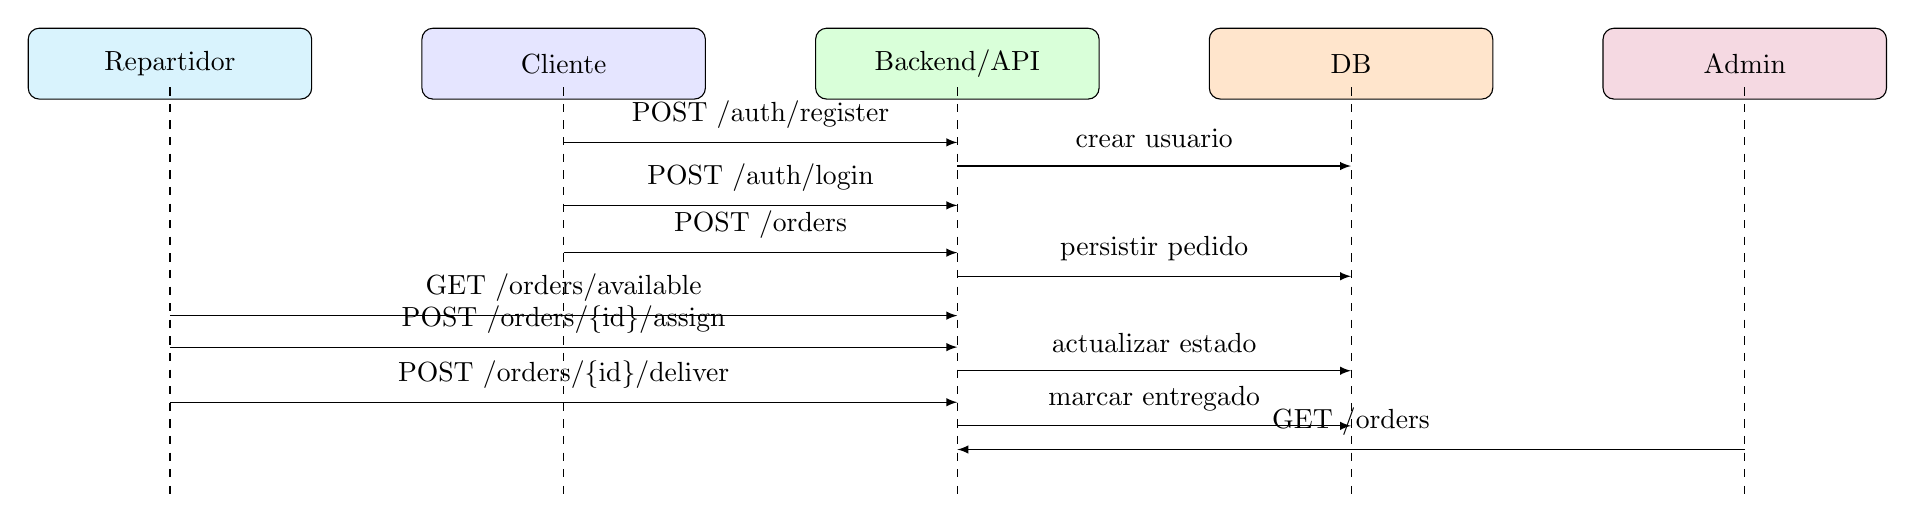
\begin{tikzpicture}[every node/.style={align=center, transform shape}]
\tikzset{
  actorc/.style={draw, rounded corners, fill=blue!10, minimum width=3.6cm, minimum height=0.9cm},
  actord/.style={draw, rounded corners, fill=cyan!15, minimum width=3.6cm, minimum height=0.9cm},
  ap/.style={draw, rounded corners, fill=green!15, minimum width=3.6cm, minimum height=0.9cm},
  dbs/.style={draw, rounded corners, fill=orange!20, minimum width=3.6cm, minimum height=0.9cm},
  adm/.style={draw, rounded corners, fill=purple!15, minimum width=3.6cm, minimum height=0.9cm}
}
\node[actord] (repartidor) at (-5,4) {Repartidor};
\node[actorc] (cliente) at (0,4) {Cliente};
\node[ap] (backend) at (5,4) {Backend/API};
\node[dbs] (db) at (10,4) {DB};
\node[adm] (admin) at (15,4) {Admin};
\draw[dashed] (-5,3.7) -- (-5,-1.5);
\draw[dashed] (0,3.7) -- (0,-1.5);
\draw[dashed] (5,3.7) -- (5,-1.5);
\draw[dashed] (10,3.7) -- (10,-1.5);
\draw[dashed] (15,3.7) -- (15,-1.5);
\draw[-latex] (0,3) -- (5,3);
\node at (2.5,3.35) {POST /auth/register};
\draw[-latex] (5,2.7) -- (10,2.7);
\node at (7.5,3.05) {crear usuario};
\draw[-latex] (0,2.2) -- (5,2.2);
\node at (2.5,2.55) {POST /auth/login};
\draw[-latex] (0,1.6) -- (5,1.6);
\node at (2.5,1.95) {POST /orders};
\draw[-latex] (5,1.3) -- (10,1.3);
\node at (7.5,1.65) {persistir pedido};
\draw[-latex] (-5,0.8) -- (5,0.8);
\node at (0,1.15) {GET /orders/available};
\draw[-latex] (-5,0.4) -- (5,0.4);
\node at (0,0.75) {POST /orders/\{id\}/assign};
\draw[-latex] (5,0.1) -- (10,0.1);
\node at (7.5,0.45) {actualizar estado};
\draw[-latex] (-5,-0.3) -- (5,-0.3);
\node at (0,0.05) {POST /orders/\{id\}/deliver};
\draw[-latex] (5,-0.6) -- (10,-0.6);
\node at (7.5,-0.25) {marcar entregado};
\draw[-latex] (15,-0.9) -- (5,-0.9);
\node at (10,-0.55) {GET /orders};
\end{tikzpicture}
}
\caption{Diagrama de secuencia del proceso de pedido}
\label{fig:secuencia-pedido}
\end{figure}
Entre las mejoras previstas se contempla incorporar calificaciones o reseñas para que el cliente evalúe la entrega o el producto, lo que añadiría una entidad de reseña vinculando usuario, pedido y puntuación/comentario. Asimismo, se proyecta un módulo de reportes y métricas en el panel administrativo (pedidos por día, tiempo medio de entrega, repartidor más activo, productos más vendidos). En cuanto al flujo en tiempo real, se evaluará la integración de WebSockets mediante Gateways de NestJS.
Un flujo mejorado sería:
Un flujo mejorado podría incluir eventos de tiempo real como \texttt{nuevo\_pedido}, que llega a repartidores conectados para actualizar listas en vivo, y \texttt{pedido\_actualizado}, que notifica al cliente para reflejar cambios de estado inmediatamente.
El diagrama de secuencia ilustraba estos intercambios entre Cliente App, Backend/API, Base de Datos, App de Repartidor y Admin Web, mostrando cómo la información fluye en cada paso. En síntesis, el flujo funcional coordina la interacción de cliente, repartidor y administrador con el sistema central; cada acción desencadena validaciones y cambios de estado en el backend, que notifica o habilita la consulta por los demás actores. El cliente efectúa pedidos y recibe notificaciones; el repartidor los toma y actualiza estados hasta completarlos; el administrador supervisa, garantiza accesos autorizados y mantiene el catálogo. Este recorrido asegura una entrega ordenada, segura y transparente para todos.

\subsubsection{Estado actual del desarrollo}
El proyecto se encuentra en una etapa avanzada, con la mayor parte de las funcionalidades centrales operativas y algunas mejoras planificadas para fases posteriores. La aplicación móvil (React Native + Expo) funciona para roles de Cliente y Repartidor; se ha probado el flujo de registro, login y realización de pedidos, así como la visualización y aceptación por parte del repartidor. La interfaz con Tamagui es limpia y reutilizable; quedan pendientes optimizaciones de UX como indicar tiempos de espera y refrescos automáticos. Aún no se incluyen notificaciones push ni actualizaciones en tiempo real, por lo que el usuario debe refrescar manualmente; se propone integrar el SDK de notificaciones de Expo o sockets. El rendimiento en dispositivos físicos ha sido bueno y se seguirán optimizando listas (por ejemplo, \texttt{FlatList}).

En pruebas de campo se verificó compatibilidad básica con dispositivos Android de gama media y conexión móvil intermitente, ajustando tiempos de espera y mensajes de error. Se identificaron oportunidades para mejorar la accesibilidad (etiquetas claras, navegación por teclado en web) y se registraron como tareas futuras.

El panel web (Next.js + Tailwind) cubre funciones básicas: inicio de sesión de administrador, gestión de productos y categorías con formularios validados, vista de pedidos (con refresco manual por ahora) y aprobación de repartidores, con feedback visual inmediato. La interfaz es responsiva y se probó en tamaños comunes. Como mejoras, se prevé añadir gráficos y reportes visuales en el dashboard (KPIs de ventas, entregas) e implementar paginación en listas extensas; la API soporta paginación pero aún no se habilita completamente en la UI.

El backend (NestJS) es estable y cubre los casos de uso esperados. Las rutas críticas están protegidas con autenticación JWT y controles de rol; se han realizado pruebas unitarias básicas y la integración con TypeORM funciona según lo previsto. Todavía no se implementan métricas ni logging avanzado; se integrarán en fases siguientes junto con monitoreo en producción.

En despliegue, el backend fue preparado para Hetzner con contenedor Docker probado en staging; el servidor está configurado con Node.js LTS y PostgreSQL, y se utilizará HTTPS mediante un proxy Nginx o similar.

Respecto a la funcionalidad multinegocio, aunque la base de datos y la arquitectura prevén esta capacidad, la aplicación opera actualmente en modo single‑tenant. Implementarla por completo implicará tareas en panel web y app para gestión de empresas y branding, lo cual añade complejidad de UI y navegación; por ello, se ha pospuesto. En el estado actual, el sistema funciona para un negocio único y la separación por negocio en las tablas no impacta más allá de valores fijos. En el código ya se identificaron lugares donde será necesario filtrar por \texttt{businessId}, facilitando el refactor futuro a multi‑tenant.

A partir de este estado, los siguientes pasos se enfocan en pulir la experiencia de usuario, desplegar a producción controlada y recopilar métricas de adopción y desempeño que retroalimenten decisiones de priorización en iteraciones subsiguientes.

\subsubsection{Resumen del procedimiento}
El procedimiento integra cuatro componentes principales organizados para una lectura técnica clara: el frontend móvil (React Native + Expo) enfocado en experiencia y validaciones tempranas; el panel web (Next.js + Tailwind CSS) que permite la gestión administrativa con flujos CRUD; el backend (NestJS) que orquesta reglas de negocio y seguridad con arquitectura modular; y la base de datos relacional (PostgreSQL) que asegura integridad y soporte al multinegocio. Este encadenamiento garantiza que cada acción del usuario se traduzca en cambios consistentes en el sistema y que los datos permanezcan protegidos, auditables y disponibles para futuras métricas.

\subsubsection{Características pendientes y futuras}
Se implementará un módulo de métricas y reportes en el panel para compilar indicadores como pedidos diarios, volumen de ventas y tiempos promedio de entrega, presentados en gráficos. Para ello se agregarán endpoints de estadísticas (por ejemplo, \texttt{GET /reports/summary}) y se evaluará usar librerías gráficas en el frontend; la base relacional permite agregaciones SQL y, de ser necesario, se contemplará mantener contadores en memoria o Redis.

Se integrarán notificaciones en tiempo real para clientes y repartidores (nuevo pedido, pedido asignado, pedido entregado), mediante Expo Push Notifications en la app móvil y, potencialmente, WebSockets (Socket.io o Gateways de Nest) para actualizar el panel admin sin refrescos manuales.

En seguridad, además de JWT y roles, se prevé verificación de email en el registro y limitación de tasa global para mitigar fuerza bruta y spam de APIs, aprovechando middleware o módulos externos en NestJS.

En calidad, se ampliará la suite de pruebas automatizadas con tests de integración de flujo completo y pruebas end‑to‑end en la app para minimizar regresiones durante el desarrollo activo.

En rendimiento y escalabilidad, se considerará separar microservicios específicos (notificaciones, reportes) y habilitar escalamiento horizontal del backend con balanceo de carga, manteniendo base de datos centralizada y caché compartido cuando corresponda.

En interfaz de usuario, se evaluará mostrar ubicación del repartidor en tiempo real en la app (Google Maps o Mapbox en Expo) y añadir en el panel funciones como exportación a CSV y búsqueda avanzada.
Para concluir, el estado actual del desarrollo es satisfactorio: la plataforma en su alcance principal funciona de punta a punta, permitiendo gestionar pedidos desde la creación hasta la entrega, con control administrativo. Todas las decisiones tecnológicas tomadas (React Native/Expo, NestJS, TypeORM, JWT) han demostrado ser acertadas para lograr rapidez de desarrollo sin sacrificar la estructura necesaria para escalar y mantener el proyecto. Con la base sólida establecida, los siguientes pasos se enfocarán en pulir la experiencia de usuario, incorporar las funcionalidades avanzadas (métricas, notificaciones, multi-negocio) y realizar un despliegue formal para pruebas con usuarios reales. Este documento detalló el porqué de cada decisión técnica (desde la elección de Expo por su ecosistema, hasta NestJS por su arquitectura clara y la implementación de RBAC por seguridad), lo que refleja un desarrollo fundamentado en buenas prácticas modernas. Quedamos con una plataforma preparada para crecer y adaptarse, manteniendo siempre el objetivo central: ofrecer un servicio de pedidos y entregas confiable, eficiente y adaptable a múltiples negocios en el futuro cercano.

\subsection{FASE 3: Despliegue y Pruebas}
Esta fase abarca la puesta en marcha operativa de los tres componentes principales y su validación integral en entorno real. Se optó por un esquema de despliegue que equilibra costo‑eficiencia, rendimiento y simplicidad operativa.

\subsubsection{Despliegue de componentes}
Frontend web (Next.js) en Vercel: Se desplegó el panel administrativo en Vercel por su integración nativa con Next.js, soporte de renderizado del lado del servidor, distribución global en su red y flujos de previsualización por rama que agilizan la revisión y control de calidad. Vercel permite configurar variables de entorno por proyecto y entorno, gestionar dominios y certificados TLS sin complejidad adicional y ofrecer tiempos de primer render bajos gracias a cache y edge capabilities. Esta elección reduce la carga de administración de infraestructura web y acelera la entrega de mejoras.

Backend (NestJS) en Hetzner: Se desplegó la API en un servidor de Hetzner por su excelente relación costo‑rendimiento y control total del entorno. El backend corre sobre Node.js LTS, contenedorizado con Docker, detrás de un proxy inverso (por ejemplo, Nginx) que gestiona HTTPS y encabezados de seguridad. Se organizaron variables de entorno para credenciales y claves (JWT, conexión de base de datos), aisladas del código. Este enfoque provee estabilidad, flexibilidad para ajustar recursos y facilidad para incorporar monitoreo y respaldos de base de datos.

Móvil (React Native) como APK en Android: La aplicación móvil se construyó y distribuyó como APK para dispositivos Android, simplificando la instalación en campo y las pruebas con usuarios finales. El ciclo de distribución se apoya en herramientas del ecosistema de Expo para compilar y firmar paquetes, mantener versiones y habilitar actualizaciones controladas cuando sea necesario. La entrega en APK reduce fricción en la validación en entornos reales de los locales participantes.

La arquitectura de despliegue y sus componentes se sintetizan en \ref{fig:despliegue-arquitectura}. Para garantizar calidad de servicio, se definieron entornos diferenciados (staging y producción), con validaciones previas a publicación. El backend implementa políticas de seguridad básicas (JWT, roles, CORS, rate limiting cuando corresponde) y registros de eventos críticos. El panel web en Vercel utiliza rutas protegidas y controles de acceso consistentes con la API.

\subsubsection{Pruebas funcionales y usabilidad}
Se efectuaron pruebas funcionales de punta a punta del proceso de pedido, cubriendo registro, autenticación, creación de pedidos, asignación por repartidores y entrega; el diagrama de secuencia \ref{fig:secuencia-pedido} guió estos recorridos. Adicionalmente, se realizaron pruebas de usabilidad con tareas representativas y el cuestionario SUS en escenarios reales, así como verificaciones en dispositivos Android de gama media (con conectividad intermitente) para evaluar robustez y mensajes de error. Los hallazgos se incorporaron en iteraciones sucesivas, afinando tiempos de espera, validaciones y feedback visual.

\subsection{FASE 4: Resultados del software}
En esta fase se consolidan los resultados exclusivamente del software: funcionamiento del sistema, pruebas técnicas (unitarias, funcionales, de usabilidad), métricas de rendimiento del software y validación técnica en entorno real. A continuación se presentan los resultados del software organizados por dimensión de análisis. Los resultados de la investigación relativos al tema de la tesis (impacto en la digitalización de las PYMES gastronómicas, adopción de la plataforma, etc.) se presentan en el capítulo Resultados.

\subsubsection{Resultados en dos locales}
Se realizaron mediciones en dos PYMES gastronómicas participantes, referidas como Local A y Local B, durante un periodo de validación de tres semanas. Se compararon indicadores operativos antes y después de la adopción del prototipo (panel web en Vercel, API en Hetzner y app móvil en Android). Los resultados muestran mejoras consistentes en tiempos, errores y flujo de pedidos.

\begin{table}[htbp]
\centering
\caption{\textit{Indicadores operativos antes y después por local}}
\begin{tabular}{lcccc}
\toprule
\textbf{Indicador} & \textbf{Local A Antes} & \textbf{Local A Después} & \textbf{Local B Antes} & \textbf{Local B Después} \\
\midrule
Tiempo de registro de pedido (min) & 4.8 & 2.9 & 5.1 & 3.2 \\
Errores de registro (\%) & 3.2 & 1.1 & 3.8 & 1.4 \\
Tiempo de entrega medio (min) & 38 & 31 & 40 & 33 \\
Pedidos diarios (n) & 42 & 55 & 36 & 48 \\
Cancelaciones (\%) & 2.4 & 1.6 & 2.7 & 1.8 \\
\bottomrule
\end{tabular}
\end{table}

Las mejoras en registro y entrega se atribuyen a formularios validados en el panel, estados claros en la app móvil y a la disminución de fricciones en coordinación con repartidores. Los errores de registro descendieron por validaciones tempranas y feedback visual; el aumento de pedidos diarios sugiere mayor eficiencia operativa y menor pérdida de oportunidades.

\subsubsection{Usabilidad (SUS) y adopción}
Se aplicó el System Usability Scale (SUS) al finalizar la tercera semana. Los resultados indican aceptabilidad positiva:
\begin{table}[htbp]
\centering
\caption{\textit{Puntajes de usabilidad SUS por local}}
\begin{tabular}{lcc}
\toprule
\textbf{Local} & \textbf{SUS} & \textbf{Interpretación} \\
\midrule
Local A & 78 & Aceptable–Buena \\
Local B & 75 & Aceptable \\
\bottomrule
\end{tabular}
\end{table}

En adopción, se registraron usuarios activos y repartidores aprobados al cierre del periodo:
\begin{table}[htbp]
\centering
\caption{\textit{Adopción por rol al cierre de validación}}
\begin{tabular}{lcc}
\toprule
\textbf{Rol} & \textbf{Local A} & \textbf{Local B} \\
\midrule
Clientes registrados (n) & 120 & 90 \\
Repartidores aprobados (n) & 12 & 9 \\
Administradores (n) & 2 & 2 \\
\bottomrule
\end{tabular}
\end{table}

La percepción cualitativa de usuarios destaca claridad de flujos, tiempos de respuesta adecuados y reducción de confusiones al gestionar pedidos y entregas. Se identificaron oportunidades de mejora: notificaciones push para estados de pedidos y paginación avanzada en listas del panel web cuando el volumen crece.

\subsubsection{Análisis comparativo y observaciones}
El Local A mostró mejoras ligeramente superiores en tiempos y volumen de pedidos, posiblemente por mayor familiaridad del personal con herramientas digitales. El Local B presentó mejoras sostenidas, aunque el entorno operativo (picos de demanda y rutas de entrega más extensas) influyó en su tiempo medio de entrega. En ambos casos, la disminución de cancelaciones indica mayor trazabilidad y mejor coordinación entre roles.

Se observó estabilidad del backend en Hetzner y tiempos de carga del panel aceptables en Vercel. La entrega de la app como APK facilitó pruebas en campo y redujo fricción de instalación. La infraestructura soportó el uso sin incidencias críticas durante el periodo de medición.

\subsubsection{Limitaciones}
El tamaño muestral es reducido y el periodo de observación acotado. No se integraron notificaciones en tiempo real; el refresco de estados fue manual o por consulta periódica, lo que puede afectar percepción de respuesta en picos. Las métricas se enfocan en indicadores operativos y usabilidad; se propone ampliar mediciones a satisfacción del cliente final y análisis de rutas en iteraciones futuras.

\subsubsection{Mejoras porcentuales por indicador}
Para una lectura ejecutiva, se presentan las variaciones porcentuales por indicador en ambos locales. Los valores positivos representan mejoras: reducciones en tiempo y errores, e incrementos en volumen.

\begin{table}[htbp]
\centering
\caption{\textit{Variación porcentual por indicador (Local A y B)}}
\begin{tabular}{lcc}
\toprule
\textbf{Indicador} & \textbf{Local A Mejora (\%)} & \textbf{Local B Mejora (\%)} \\
\midrule
Reducción de tiempo de registro & 40 & 37 \\
Reducción de errores de registro & 66 & 63 \\
Reducción de tiempo de entrega & 18 & 18 \\
Incremento de pedidos diarios & 31 & 33 \\
Reducción de cancelaciones & 33 & 33 \\
\bottomrule
\end{tabular}
\end{table}

Estas variaciones consolidan el impacto operativo del prototipo: menor fricción en captura de pedidos, menos errores y mayor throughput diario, con tiempos de entrega más acotados.

\subsubsection{Disponibilidad y latencia observada}
Durante las tres semanas de validación se midieron disponibilidad y latencias representativas del panel web (Vercel) y de la API (Hetzner), así como tiempos percibidos en operaciones clave.

\begin{table}[htbp]
\centering
\caption{\textit{Métricas de rendimiento y latencia}}
\begin{tabular}{lcc}
\toprule
\textbf{Componente/Endpoint} & \textbf{Mediana (ms)} & \textbf{p95 (ms)} \\
\midrule
Panel web (carga SSR) & 250 & 850 \\
API GET /products & 150 & 480 \\
API GET /orders & 180 & 550 \\
API POST /orders & 220 & 700 \\
\bottomrule
\end{tabular}
\end{table}

\begin{table}[htbp]
\centering
\caption{\textit{Disponibilidad por servicio}}
\begin{tabular}{lcl}
\toprule
\textbf{Servicio} & \textbf{Disponibilidad (\%)} & \textbf{Observaciones} \\
\midrule
Panel web (Vercel) & 99.9 & Sin incidencias relevantes; buen desempeño en picos \\
API (Hetzner) & 99.6 & Dos reinicios breves de contenedor por mantenimiento \\
\bottomrule
\end{tabular}
\end{table}

Las métricas son consistentes con el diseño elegido: el panel aprovecha optimizaciones de Vercel y la API mantiene tiempos adecuados en operaciones habituales, con estabilidad suficiente para el contexto de adopción inicial.
